\chapter{Complementos de Scrum}
% Malas prácticas, consejos, tecnicas complementarias, casos de estudios

%Técnicas para requerimientos
% Historias de usuarios
% Técnica Killen 
% Mapas de historia
%Técnicas de Planeación
%Técnicas de estimación
% Poker de planeación
%Técnicas de Comunicación
% Radiadores de información
% Scrum task board
% Comunicación osmótica


\section{Técnicas de Comunicación}

\subsection{Scrum kanban board}

El Scrum kanban board es una técnica que consiste en utilizar un tablero Kanban (ver version \ref{fig:ScrumKanbanBoard}), como irradiador de información, para el manejo del cilo de estados de las tareas y de los impedimentos. El tablero Kanban debe ser visible por todo el equipo y por lo tanto transparente para todos los involucrados. Por ejemplo, durante una Daily Scrum todo el mundo es capaz de ver qué tareas se resuelven, cuáles no se han abordado todavía y qué impedimentos existen.

\begin{figure}[h]
  \centering
  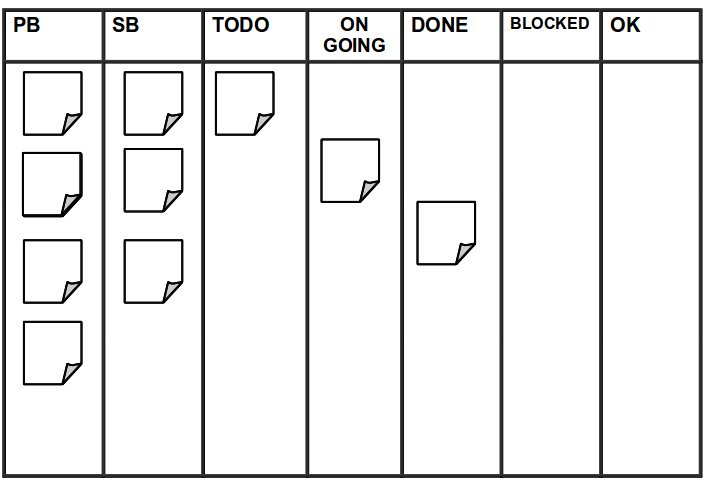
\includegraphics[scale=0.5]{ScrumKanbanBoard}
  \caption{Tablero Kanban para Scrum}
  \centering
  \label{fig:ScrumKanbanBoard} %\ref{fig:ScrumKanbanBoard}
\end{figure}


\section{Malas prácticas}

Existen muchas causas diversas de que se fracase en la implementación de Scrum. A esas acciones causas resultado de prácticas y que perjudican el buen funcionamiento de Scrum las podemos llamar malas prácticas y constituirán prácticas que se aconseja evitar.
A continuación se listan algunas de ellas:

\begin{enumerate}

\item \textbf{Aplicar mal la metodología}

Una mala práctica es aplicar mal o en forma incompleta una metodología o técnica determinada. Por ejemplo, se critica a la metodología de cascada (Waterfall) o desarrollo en cascada porque se dice que no funciona, sin embargo lo que suele suceder es que no se aplica realmente (Masa Maeda \footnote{Masa K Maeda es PhD, Founder and CEO de Valueinnova USA (capacitación Scrum). Es el creador de Serious LeAP, consultor senior del Cutter Consortium en Boston, miembro del comité de dirección del Agile Testing Alliance y maestro en la Universidad de California en Berkeley. Es pionero de Lean y Kanban para trabajo de conocimiento y uno de los formadores del Lean Kanban University. Es una figura líder mundial en Agile y ha generado Serious Games de alto calibre.}). El problemas no es que no sirva o no funcione, sino que no lo hacemos bien (Masa Maeda  2012). Pues, en el artículo original de 1970 en el que Royce Winston expone el desarrollo en cascada se habla de ciclos y de “fases sucesivas de desarrollo iterativo” \cite{Winston-Royce-1970} ofreciendo unos consejos a seguir, cosa que no se suele hacer y se da por hecho que cascada no sirve. Algo parecido ocurre con Scrum. Hay quienes dicen:  "Scrum fracasó". Pero, sin embargo, lo que suele suceder es que se dice que se implementa Scrum aunque, en la práctica, no se cumplen sus recomendaciones o se hacen hibridaciones con otras metodologías que dan como resultado algo que no es Scrum. Creyendo hacer Scrum, muchas no han logrado superarlo \cite{Gantthead-James-2010}. 

\item \textbf{Aplicar mal un principio}

En ocaciones en que se aplica mal una metodología se puede deber a mal interpretar sus principios rectores, a generalizarlos o a caer en un una especie de fundamentalismo. Por ejemplo, si consideramos el "trabajo empírico" como algo fundamental, pero basándonos en ello pretendemos que todo trabajo se base en la experiencia directa de los desarrolladores (tipo prueba error) sin recurrir a experiencias previas, a memoria histórica, a procesos organizacionales o a conocimiento teórico. De este modo se puede caer en ser un equipo de trabajo reactivo, ciego de las consecuencias a largo plazo de sus acciones e ineficiente. No es necesario reinventar la rueda cada vez que se nos presenta la necesidad de usar una y a veces eso es lo que ocurre cuando se abusa del trabajo basado en la prueba y el error. Por otro lado, cuando nuestros actos tienen consecuencias que trascienden el horizonte de aprendizaje (nuestra experiencia cercana), se vuelve imposible aprender de la experiencia directa \cite{Peter-Senge-1990}. 
En ocaciones, por poner otro ejemplo, se hace énfasis en el coraje. Pero se puede caer en ser heroico, cuando como dice una frase: "el programador heroico a menudo no ve el gran dragón" (Software Architect Bootcamp). Pues fomentar el coraje no es fomentar necesariamente las acciones individuales heroicas en vez de buscar sentirse apoyados y tener más recursos a disposición para promover el coraje para enfrentar desafíos más grandes.

\item \textbf{No hacer ingeniería por aplicar una metodología}

Metodologías como Scrum  no establecen las prácticas específicas de ingeniería, por lo que se puede aplicar la metodología sin hacer ingeniería. En este caso los ScrumMasters son responsables de promover un mayor rigor de la aplicación de las practicas ingenieriles y de la definición de “terminado” (DoD) acorde al marco de ingeniería \cite{Gantthead-James-2010}.

\item \textbf{No se cambia de mentalidad}

A veces se implementa y usa una nueva metodología pero no se cambia de forma de pensar. Es que se puede considerar que la simple adopción de una herramienta de trabajo, sin una transformación personal que la acompañe, no sirve de nada, por ejemplo adoptar Scrum sin una transformación personal \cite{Martin-Alaimo-Kleer-2014}. 

La gran mayoría de metodologías tienen detrás principios y maneras de pensar. Pues hay que entender que no se trata solo de fórmulas, sino también de formas de razonar. No se puede pretender trabajar en un equipo con alguna metodología ágil que implementa auto-organización si no se cree en la auto-organización. Hay personas que creen en el liderazgo centralizado y autoritario y no cambian su perspectiva y en vez de adaptarse a la nueva manera de trabajar terminan queriendo adaptar la manera de trabajar a su idea original, por ejemplo a la conducción centralizada y autoritaria. Esta actitud termina por generar malas prácticas que socaban el buen funcionamiento de una metodología determinada.

\item \textbf{Disociación entre producción y resto de la organización}

La disociación entre producción y resto de la organización se da cuando se implementa Scrum solo en el área de producción para hacer Scrum en el proceso de desarrollo, pero la gestión estratégiga o las capas de gestión de alto nivel de la compañía desconocen la filosofía Scrum y gestionan los portfolios, programas y proyectos con las metodologías criticadas por Scrum. Algo semejante sucede con los vendedores de la organización. Pues, si los mismos venden productos especificados de antemano y en base a esas ventas se realizan compromisos contractuales rígidos y se exije que el área de producción cumpla con esos compromisos, por más que el área de producción intente usar Scrum se puede caer en los mismos problemas que Scrum critica e incumplir con el o los proyectos.


\end{enumerate}
